%for a more compact document, add the option openany to avoid
%starting all chapters on odd numbered pages
\documentclass[12pt]{cmuthesis}

% This is a template for a CMU thesis.  It is 18 pages without any content :-)
% The source for this is pulled from a variety of sources and people.
% Here's a partial list of people who may or may have not contributed:
%
%        bnoble   = Brian Noble
%        caruana  = Rich Caruana
%        colohan  = Chris Colohan
%        comar    = Cyrus Omar
%        jab      = Justin Boyan
%        josullvn = Joseph O'Sullivan
%        jrs      = Jonathan Shewchuk
%        kosak    = Corey Kosak
%        mjz      = Matt Zekauskas (mattz@cs)
%        pdinda   = Peter Dinda
%        pfr      = Patrick Riley
%        dkoes = David Koes (me)

% My main contribution is putting everything into a single class files and small
% template since I prefer this to some complicated sprawling directory tree with
% makefiles.

% some useful packages
\usepackage{fullpage}
\usepackage{graphicx}
\usepackage{amsmath}
\usepackage{amssymb}
\usepackage[numbers,sort]{natbib}
\usepackage[backref,pageanchor=true,plainpages=false, pdfpagelabels, bookmarks,bookmarksnumbered,
%pdfborder=0 0 0,  %removes outlines around hyper links in online display
]{hyperref}
\usepackage{subfigure}
\usepackage{xspace}

%% custom fonts

\usepackage{fontspec}
\usepackage{xeCJK}

\setmainfont{Charter}[
	Path = ./fonts/,
	UprightFont = XCharter-Roman.otf,
	BoldFont = XCharter-Bold.otf,
	ItalicFont = XCharter-Italic.otf,
	BoldItalicFont = XCharter-BoldItalic.otf
	]
%\setmainfont{Utopia}[
%	Path = ./fonts/,
%	UprightFont = UtopiaStd-Regular.otf,
%	BoldFont = UtopiaStd-Semibold.otf,
%	ItalicFont = UtopiaStd-Italic.otf,
%	BoldItalicFont = UtopiaStd-SemiboldIt.otf
%	]

\setCJKmainfont{HeiseiMinStd-W5}[Path = ./fonts/]

% Approximately 1" margins, more space on binding side
%\usepackage[letterpaper,twoside,vscale=.8,hscale=.75,nomarginpar]{geometry}
%for general printing (not binding)
\usepackage[letterpaper,twoside,vscale=.8,hscale=.75,nomarginpar,hmarginratio=1:1]{geometry}

% Provides a draft mark at the top of the document.
\draftstamp{\today}{DRAFT}

\begin{document}
\frontmatter

%initialize page style, so contents come out right (see bot) -mjz
\pagestyle{empty}

\title{ %% {\it \huge Thesis Proposal}\\
{\bf Practical Concurrency Testing} \\
\normalsize \vspace{1em}
\begin{tabular}{c}
{\em or, How I Learned to Stop Worrying and Love the Exponential Explosion}
\end{tabular}}
\author{Ben Blum}
\date{Decembruary 2018}
\Year{2018}
\trnumber{}

\committee{
Garth Gibson, Chair \\
David A. Eckhardt \\
Brandon Lucia \\
Haryadi Gunawi, University of Chicago
}

\support{}
\disclaimer{}

% copyright notice generated automatically from Year and author.
% permission added if \permission{} given.

\keywords{landslide terminal, baggage claim, ground transportation, ticketing}

\maketitle

\begin{dedication}
For Elsie, Margie, Johnny, Mel, Eve, and David, who brought me here today.
\end{dedication}

\pagestyle{plain} % for toc, was empty

%% Obviously, it's probably a good idea to break the various sections of your thesis
%% into different files and input them into this file...

\begin{abstract}
Concurrent programming presents a challenge to students and experts alike because of the complexity of multithreaded interactions and the difficulty to reproduce and reason about bugs.
Stateless model checking is a concurrency testing approach which forces a program to interleave its threads in many different ways, checking for bugs each time.
This technique is powerful, in principle capable of finding any nondeterministic bug in finite time,
but suffers from exponential explosion as program size increases.
Checking an exponential number of thread interleavings is not a practical or predictable approach for programmers to find concurrency bugs before their project deadlines.

In this thesis, I develop several new techniques to make stateless model checking more practical for human use.
I have built Landslide, a stateless model checker specializing in undergraduate operating systems class projects.
Landslide extends the traditional model checking algorithm with a new framework for automatically managing
%the exploration of
multiple state spaces according to their estimated completion times,
which I show quickly finds bugs should they exist and also quickly verifies correctness otherwise.
I evaluate Landslide's suitability for inexpert use by presenting the results of many semesters providing it to students in 15-410, CMU's Operating System Design and Implementation class,
and more recently, students in similar classes at the University of Chicago and Berkeley.
%Finally, I will present several new techniques that allow stateless model checking to be practically employed on real-world programs.
%Finally, I will explore broader impact by extending Landslide to test some real-world programs and to be used by students at other universities.
Finally, I extend Landslide with a new concurrency model for hardware transactional memory,
and evaluate several real-world transactional benchmarks to show that stateless model checking can keep up with the developing concurrency demands of real-world programs.
\end{abstract}

\begin{acknowledgments}
% things to thank
% stimhack
% csd bgames
% undergrad frenz
% new frenz
% 410 ta community
% emarhavil
%
% \\

I thank my dog, Louie.
\end{acknowledgments}

\tableofcontents
% TODO: figure out how to make latex abbreviate these
\listoffigures
\listoftables

\mainmatter

%% Double space document for easy review:
%\renewcommand{\baselinestretch}{1.66}\normalsize

% The other requirements Catherine has:
%
%  - avoid large margins.  She wants the thesis to use fewer pages,
%    especially if it requires colour printing.
%
%  - The thesis should be formatted for double-sided printing.  This
%    means that all chapters, acknowledgements, table of contents, etc.
%    should start on odd numbered (right facing) pages.
%
%  - You need to use the department standard tech report title page.  I
%    have tried to ensure that the title page here conforms to this
%    standard.
%
%  - Use a nice serif font, such as Times Roman.  Sans serif looks bad.
%
% Other than that, just make it look good...

\newcommand\simics{\textsc{Simics}}
\newcommand{\sect}[1]{\S #1}
\newcommand\hilight[2]{\color{#1}#2\color{black}}
\definecolor{orange}{RGB}{192,96,0}
\definecolor{olivegreen}{RGB}{0,127,0}
\definecolor{brickred}{RGB}{192,0,0}
\definecolor{commentblue}{RGB}{0,0,192}

\newtheorem{theorem}{Theorem}

\newcommand\llama[1]{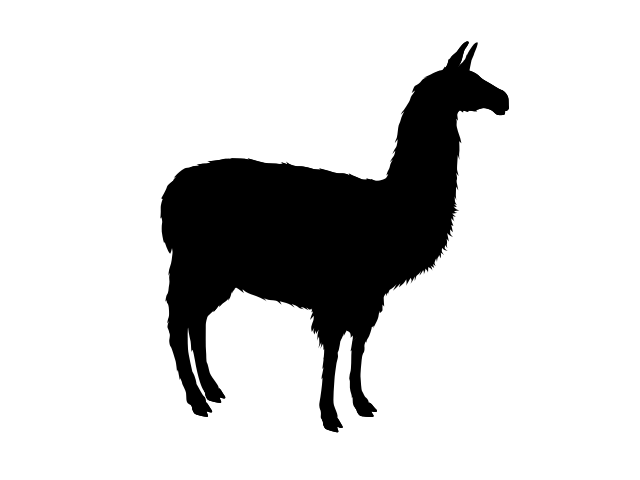
\includegraphics[width=#1]{llama.pdf}}
\newcommand\llitem{\item[\llama{1.2em}]}

\newcommand{\inspirationallinebreak}{\vspace{0.25em}}
\newcommand{\inspirationalhyphen}{-\hspace{-0.15em}-\xspace}
\newcommand\inspirationalquote[2]{\begin{flushright}
	\vspace{-1em}
	{
	\fontspec[Path=./fonts/]{AlexaStd}
	{\em #1}
	\inspirationallinebreak

	-\hspace{-0.15em}-\hspace{-0.15em}-{#2}
	}
	\vspace{2em}
\end{flushright}}

\chapter{Introduction}
\inspirationalquote{
\begin{tabular}{p{0.7\textwidth}}
Please hold on. This thesis will be departing shortly for the Landslide terminal, baggage claim, ground transportation, and ticketing.
\end{tabular}}
{Pittsburgh International Airport (paraphrased)}

\revision{Pick up any recent concurrency-related research paper, %from the last few decades,
and chances are its very first sentence will tell you
%how notoriously difficult concurrency bugs are compared to sequential ones
that concurrency bugs are notoriously difficult to find, reproduce, diagnose, and/or fix
% ,
%and/or thereafter verify fixed,
%compared to sequential ones,
%on account of the multitude of thread interleavings one must test
\cite{nidhugg,optimal-dpor,coredet,sealing,quicksand,landslide,this-thesis,concuerror,
%cspec, % 2nd sentence in cspec >_>
bpor,
%parrot, % 2nd sentence in parrot
peregrine,
%bugtm, % 1st and 2nd sentence
satcheck,
racerx,
%ifrit, % 1st para, approx
datacollider,
fasttrack,
mcr-tsopso,
mcr,
macemc,
contessa,
%lvish, % "it must become easier"
dthreads,
taxdc,
%learning-from-mistakes, % sentence 3ish
avio,
symbiosis,
chess-icb,
chess,
recordreplaydrs,
kendo, % first WHOLE PARAGRAPH geez dude
%hybriddatarace, % 3rd sentence
parallel-dpor,
%eraser, % 3rd sentence 2nd paragraph
%racefuzzer, % 2nd sentence
%tsan, % 2nd sentence
sully-thesis,
%compcerttso, % 2nd sentence
modist,
maple,
simtester}.
%compared to sequential programming.
%
%Indeed, just as conditional statements and loops introduce additional possible program behaviours
%depending on different input,
%concurrent execution introduces additional possible behaviours even under a fixed input.
%Unlike input nondeterminism,
%concurrency nondeterminism typically manifests at the whims of chance,
%making bug-finding and verification especially challenging.
%
%What is a concurrency bug, and
How could a single programming technique be so troublesome
as to inspire multiple decades of verification research?
Allow me to begin this thesis by answering this question
in layperson's terms,
using two parables.

My favourite way to explain concurrency to a non-technical audience
%(e.g., family members)
is by analogy with unlocking car doors.
In many %makes and
models of cars, the door handle and locking mechanism are intertwined
in such a way that the door cannot unlock while its handle is being pulled~\cite{car-doors}.
Most car users, then,
%are familiar with
have suffered the experience of
trying to open the passenger door
at exactly the same moment as the driver turns the key in the lock:
%not only does the door not open, but
it fails to unlock, and
they must beseech the driver to turn the key again!
If they had pulled the handle any later, it would have opened as normal;
any earlier, and it would have been as though not having the key at all,
but would at least have unlocked properly at the first turn of the key later.
This violation of expected behaviour -- that the key need not be turned twice --
is a {\em bug},
and its dependence on the two travelers' actions {\em interleaving}
%with the driver's actions
in a particular way
makes it a {\em concurrency bug}.
This example involves only three events (pulling the handle, releasing the handle, and turning the key),
but what of a system with hundreds or thousands of times more?
Unfortunately, the number of possible interleavings grows {\em exponentially} with the number of events.

%Exponential explosion is easily understood through the tale of Sissa Ibn D\`{a}hir
The Islamic historian Ibn Khallik\={a}n told perhaps the first cautionary tale of exponential explosion
\cite{ibn-khallikan,khallikān1868ibn}.
Sissa Ibn D\`{a}hir,
credited with the invention of chaturanga (the precursor to modern chess),
was invited by King Shihr\^{a}m to request any reward he desired.
Sissa requested that a grain of wheat be placed on the first square of a chessboard,
two in the second, and so on, doubling the number of grains in each previous square until all 64 be filled.
The king at first laughed, thinking it a pittance,
realizing only later that to fulfill this would require
more than all the wheat in all the cities on Earth.
Modern programmers will recognize this sum as $2^{64}-1$,
the largest value representable by an unsigned 64-bit integer,
or approximately 18 billion billion.
The number of interleavings in a concurrent system grows at a similarly intractable rate
(although not necessarily exactly doubling each time),
with the number of chessboard squares filled with grain corresponding to the number of events in a program's execution.
A concurrency bug, then, is a single poisoned grain of wheat,
which must be rooted out from the stock before feeding the townspeople.
And Sissa himself is the programmer,
whose software is invariably large enough to be far beyond the reach of any exhaustive verification strategy.
}

\section{Motivation}

To take advantage of multiple cores for performance, programmers must write software to execute {\em concurrently} --
using multiple {\em threads} which execute multiple parts of a program's logic simultaneously.
However, when threads access the same shared data, they may interleave in unexpected ways which change the outcome of their execution.
When an unexpected interleaving produces undesirable program behaviour,
for example, by corrupting shared data structures,
we call it a {\em concurrency bug}.
Concurrency bugs are notoriously hard for programmers to find and debug
because the specific thread interleaving required to trigger them arises at random during normal execution,
and often with very low probability.
%Concurrency bugs are notoriously hard to find and reproduce because they only appear in specific thread interleavings, which arise at random during normal program execution.
% TODO(LAYMAN): give example of trying to open car door at same time as friend turns key to unlock it.

Most commonly, a programmer searches for concurrency bugs in her code by running it many times (in parallel, in serial, or both),
hoping that eventually, it will run according to the particular interleaving required to expose a hypothetical bug.
This technique, known as {\em stress testing}, is unreliable,
providing no guarantee of finding the failing interleaving in any finite amount of time.
It also provides no assurance of correctness:
when finished, there is no way of knowing how many distinct thread interleavings were actually tested.
Nevertheless, stress testing remains popular because of how easily a programmer can use it:
she simply wraps her program in a loop, sets it to run overnight, and kills it if her patience runs out before it finds a bug.

{\em Stateless model checking} \cite{verisoft} is an alternative way to test for concurrency bugs,
or to verify their absence,
which provides more reliable coverage, progress, and verification than stress testing.
A stateless model checker tests a program by forcing it to execute a new unique thread interleaving on each iteration of the test,
capturing and controlling the randomness in a finite state space of all possible interleavings.

Unfortunately, the size of these state spaces is exponentially proportional to the size of the tested program.
% TODO(LAYMAN): explain exponential explosion by relating the parable of grains of rice on a chessboard.
For even moderately-sized programs, there may be more possible ways to interleave every thread's every instruction
than particles in the universe.
Accordingly, a programmer who wants her test to make reasonable progress through the state space must choose a subset of ways that her threads could interleave,
focusing on fully testing that subset, while ignoring other possibilities she doesn't \revisionminor{think she cares} about.
However, it is difficult to choose a subset of thread interleavings that will produce a meaningful, yet feasible test.
Until computers can automatically navigate this trade-off in some intelligent way,
programmers will continue to fall back to the random approach of stress testing.

Another problem stateless model checking suffers is that certain types of programs cannot be tested without the programmer putting forth some manual instrumentation effort.
For example, operating system kernels implement their own sources of concurrency and their own synchronization primitives,
so \revisionminor{a checker must} be told how to identify and control the execution of each thread.
Some expert concurrency research wizards may be willing to add manual annotations to their code,
but required manual effort is a serious downside for anyone with a looming deadline,
and especially so for students who are still learning basic concurrency principles.
%We should not expect programmers to add effortful manual annotations to their code,
%or they will abandon our fancy technique to instead simply run stress tests until their deadline tomorrow evening.

\section{Contributions}

This thesis will solve both problems discussed above.
My thesis statement is as follows:

\begin{center}
\begin{tabular}{p{0.8\textwidth}}
	\revisionminor{{\em Combining %both
	theoretically-founded automatic reduction techniques
	and user-informed heuristic ones,
	stateless model checking can sufficiently mitigate exponential explosion
	to be a practical testing technique for inexperienced users and real-world programs alike.}}
\end{tabular}
\end{center}

\vspace{0.75em}

I have built Landslide \cite{landslide}, a stateless model checker for thread libraries and kernels,
and I have developed some techniques for automatically choosing the best thread interleavings to test
and for automatically instrumenting operating system kernels in an educational setting.
This thesis will comprise three major contributions:

\begin{enumerate}
	\item {\bf Meaningful state spaces (\Cref{chap:quicksand}).}
		I will present {\em Iterative Deepening}, a new algorithm for navigating the trade-off in how many preemption points to test at once.
		Iterative Deepening incorporates state space estimation \cite{estimation} to decide on-the-fly whether each state space is worth pursuing, and uses data race analysis \cite{tsan} to find new preemption point candidates based on a program's dynamic behaviour.
		This section will include a large evaluation of the technique, comparing its performance to three \revisionminor{prior-work} approaches across 600+ unique tests.
		I will show that Iterative Deepening of preemption points outperforms prior work in terms \revisionminor{of both} finding bugs quickly and completely verifying correctness when no bug exists.
	\item {\bf Educational use (\Cref{chap:education}).}
		For the past five semesters, I have offered a fully-automated version of Landslide to students in 15-410, CMU's undergraduate Operating System Design and Implementation class \cite{kspec,thrlib}, for use as a debugging aid during the thread library project.
		Recently I have also extended Landslide to handle Pintos kernel projects from other universities \cite{pintos}.
		In the two most recent semesters, I collaborated with Operating Systems course staff at two such schools, the University of Chicago and University of California at Berkeley,
		to provide debugging feedback to their students.

		At all three universities I then collected statistics on the numbers and types of bugs found,
		and surveyed students to understand the human experience.
		This section will present the study's results
		to evaluate the suitability of stateless model checking in an educational setting.
	\item {\bf Hardware Transactional Memory (HTM) (\Cref{chap:tm}).}
		HTM is a relatively new concurrent programming technique \cite{htm-haswell,htm-experience}
		which is not yet addressed by modern model checkers.
		I have extended Landslide's concurrency model to support
		HTM's execution semantics and several advanced features, % abort codes p much
		%both hardware (HTM) and software (STM) variants of TM,
		and tested several ``real-world'' HTM programs and benchmarks.
		This section will discuss the theoretical techniques I used to model the new form of concurrency,
		present associated correctness proofs of my approach,
		and show the verification results.
\end{enumerate}

\section{Organization}

The rest of this dissertation is organized as follows.

\begin{itemize}
	\item {\bf Background:} \Cref{chap:background} will present the requisite background material on concurrent programming, stateless model checking, and the various types of programs targeted by Landslide.
	\item {\bf Landslide:} \Cref{chap:landslide} explains the design and implementation of Landslide
		%the core of my stateless model checking framework,
		and all the special features it's been equipped with over the years.
		It is the foundation upon which all three contributions above build.
	\item {\bf Quicksand:} \Cref{chap:quicksand} presents the Iterative Deepening framework which more intelligently chooses which state spaces to test, corresponding to contribution 1 above.
	\item {\bf Education:} \Cref{chap:education} discusses my evaluation of Landslide
		in CMU's 15-410 class environment using the Pebbles kernel,
		and in the University of Chicago's and Berkeley's OS class environments using the Pintos kernel,
		corresponding to contribution 2 above.
	%\item {\bf Pebbles:} \Cref{chap:410} discusses my evaluation of Landslide in CMU's 15-410 class environment using the Pebbles kernel, corresponding to contribution 2 above.
	%\item {\bf Pintos:} \Cref{chap:410} discusses my evaluation of Landslide in the University of Chicago's and Berkeley's OS class environments using the Pintos kernel, corresponding to contribution 2 above.
	\item {\bf Transactional Memory:} \Cref{chap:tm} presents my extension of Landslide's concurrency model to handle transactional concurrency and the evaluation thereof, corresponding to contribution 3 above.
	\item {\bf Related Work:} \Cref{chap:relatedwork} honors my neighbours and ancestors in research spirit.
	\item {\bf Future Work:} \Cref{chap:warpzone} lists stateless model checking's remaining shortcomings and how new research might address them.
	\item {\bf Conclusion:} \Cref{chap:conclusion} provides some thoughts on the future of the field.
\end{itemize}

\section{Notes on reading this thesis}

\subsubsection{Experience}

I have tried to make this document accessible to readers of all programming experience levels,
although some of the research being theoretical and several layers of abstractions deep,
I cannot promise all easy reading.
\Cref{chap:background}, Background, provides what I hope are friendly concrete examples
to help the reader feel comfortable with each level of intuition that upcoming algorithms will build upon.
These should suffice for the experiments and overall contributions,
if not necessarily the details of each algorithm or soundness proof.
In particular, \Cref{chap:education}, Education,
may be approached with no knowledge of concurrency or model checking,
taking it merely as a study of a magic new debugging tool in the classroom setting.
The more ambitious reader may proceed to the Landslide chapter's algorithm walkthroughs~(\cref{sec:landslide-algs}),
which should equip them to understand every detail herein.
Readers who are here only to skim and skip around should at least be aware of the glossary~(\cref{sec:glossary})
to help clarify any terminology confusion.

\subsubsection{Vision}

Color will be used in figures and graphs to add visual contrast and make the data easier to navigate at a glance,
but only in redundant ways also signaled by symbols.
I have made some effort to choose palettes friendly to color-blindness;
should the reader find contrasts too low anyway,
whether being color-blind or reading a physical copy printed in greyscale,
they may be assured all important distinctions still render in monochrome.
For example, ovals and rectangles typically depict different threads,
and $\dagger$ distinguishes state space estimates from completed verifications.
\revision{Should any vision-impaired reader require fully-textual figure descriptions,
I would be happy to provide them upon request.}

\subsubsection{Language}

Pronoun use will vary between more specific and more ambiguous to convey additional nuance.
The singular ``I'' is associated with my own research contributions,
while the royal ``we'' should be taken to include the reader,
such as when surveying background material or related work,
to which the author and reader share more similar relationships.
The impersonal ``the programmer'' will be referred to as she/her
to challenge readers' unconscious bias about gender in computer science,
as well as to highlight her role as the intended user, separate from the underlying research.
%to distinguish her from the thesis audience concerned with the underlying research,
Gender-neutral pronouns will be used to refer to
individual students who participated in the user studies,
%will be given the more inclusive they/them.
%Gender-neutral pronouns will also be used
as well as
on the author themself.

\subsubsection{Code}

\newcommand\landslidelicense{BSD\xspace}

This document is, in a way, only half the work of the thesis, the other half being Landslide's implementation.
While some readers may prefer to be taught in prose and/or mathematical notation how an algorithm works,
others may find that disorienting and wish to see things in a way a compiler would understand.
\revisionminor{
The Landslide codebase is open-source under the \landslidelicense license,
available at \url{https://github.com/bblum/landslide}.
\Cref{chap:landslide} provides more detail and}
serves as a guide to browsing the repository.
Later chapters will often make parenthetical references to specific files and/or functions
therein which implement a feature under discussion.

% TODO:
% Finally, this thesis also contains a small puzzle-hunt to reward dedicated readers who make it all the way through.

\newpage
\thispagestyle{empty}
\begin{center}
\begin{tabular}{c}
\vspace{12em} \\
\includegraphics[width=0.55\textwidth]{how-i-learned.png}
\end{tabular}
\end{center}

\input{background}
\chapter{Landslide}
\inspirationalquote{Somewhere is the promise of an uncharted trail, with 700 branching limbs and 700 ways to fail.}
{ThouShaltNot, "Cardinal Directions"}

Landslide is a model checker implemented as a plug-in module for x86 full-system simulators.
The program to be tested runs in a simulated environment,
and Landslide uses its access to the simulator's internal state to inspect and manipulate the memory and thread scheduling of the program as it executes.
As of this thesis's writing, Landslide supports the use of two possible simulators:

\begin{itemize}
	\item {\bf Simics} \cite{simics}, a proprietary simulator licensed commercially by Wind River, used at CMU in 15-410 to run Pebbles thread libraries and kernels, and
	\item {\bf Bochs} \cite{bochs}, an open-source (LGPL) simulator used at the University of Chicago, Berkeley, and other schools to run Pintos kernels.
\end{itemize}

% TODO: update this linkerino (repository name)
% TODO: add some backup linkeroos
The Bochs port of Landslide is likewise open-source and available at \url{https://github.com/bblum/bochs}.
% TODO: refresh
The HEAD commit at the time of writing is 8984021.
The Simics port is available upon request.

This chapter will discuss Landslide's outer and inner workings for both aspiring users and aspiring developers in all gory detail. Strap in.

\section{User interface}

This section describes the features of Landslide the average student user should expect to interact with.
% TODO: make more specific section reference
Separate user guides also exist, described in Chapter~\ref{chap:410}.

\subsection{Setup}

Two setup scripts are provided, one for each supported kernel architecture: {\tt p2-setup.sh} and {\tt pintos-setup.sh}.
The user should supply the directory containing their project implementation.
The latter script also supports arguments specifying which of the Pintos projects to target.
For example:
\begin{itemize}
	\item {\tt ./p2-setup.sh /path/to/my/p2}
	\item {\tt ./pintos-setup.sh /path/to/my/threads} (2nd argument defaults to ``{\tt threads}'')
	\item {\tt ./pintos-setup.sh /path/to/my/userprog userprog}
\end{itemize}

These scripts accomplish the following setup tasks (among other trivialities):
\begin{itemize}
	\item Copy the user's code into {\tt pebsim/p2-basecode/} or {\tt pebsim/pintos/},
		which contain a pre-annotated Pebbles reference kernel binary or pre-annotated Pintos basecode, respectively.
	\item Build the code in its new location.
	\item Run the instrumentation script on the resulting binary to let Landslide know where all the important functions are
		(see \sect{\ref{sec:landslide-glue}}).
\end{itemize}

\subsection{Running Landslide through Quicksand}
\label{sec:landslide-quicksand-options}

The preferred method of invoking Landslide is through Quicksand, the Iterative Deepening wrapper program which has all of Chapter~\ref{chap:quicksand} to itself.
% TODO: add quicksand symlink
This is done via the {\tt ./landslide} script in the top-level directory, which:
\begin{itemize}
	\item Checks if the user needs to run {\tt *-setup.sh} again, in case their source code was more recently updated than the existing annotated build (a common mistake),
	\item Passes its arguments through to {\tt id/landslide-id}, the Quicksand binary,
		and
	\item (If during the student user study,) compresses the resulting log files,
		creates a snapshot tarball of them and the current version of the user's code,
		and sends it to me for nefarious research purposes.
\end{itemize}

\subsubsection{Command-line argments}

The following command line arguments are recommended for the common user.

\begin{itemize}
	\item {\tt -p PROGRAM}: the name of the test case to invoke
	\item {\tt -t TIME}: wall-clock time limit, in seconds; or suffixed with one of {\tt ydhms} for years, days, hours, minutes, or seconds respectively (default 1h)
	\item {\tt -c CPUS}: maximum number of Landslide instances to run in parallel (defaults to half the number of system CPUs)
	\item {\tt -i INTERVAL}: interval of time between printing progress reports (default 10s)
	\item {\tt -d TRACEDIR}: directory for resulting bug traces (default current directory)
	\item {\tt -v}: verbose mode (issues output for each executed interleaving by each instance of landslide, makes progress reports more detailed, etc)
	\item {\tt -l}: leave Landslide log files from completed state spaces even when no bug was found (deleted automatically by default)
	\item {\tt -h}: print help text and exit immediately
\end{itemize}

The following ``secret'' arguments also exist, primarily for my own use in running experiments or debugging.

\begin{itemize}
	\item {\tt -C}: enable ``control experiment'' mode, i.e., run only 1 instance of Landslide, with all (non-data-race) preemption points enabled in advance
		% TODO: put a section reference here
	\item {\tt -I}: enable Iterative Context Bounding (requires {\tt -C}, although future work may relax this restriction);
		this generally causes bugs to be found faster should they exist, but degrades completion time
		(\sect{\ref{sec:landslide-icb}})
	\item {\tt -0}: enable Preempt-Everywhere mode (\sect{\ref{sec:quicksand-eval}}, requires {\tt -C})
	\item {\tt -H}: use Limited Happens-Before for data-race analysis (\sect{\ref{sec:background-hb}})
		(default for Pebbles kernelspace mode)
	\item {\tt -V}: use vector-clock-based Pure Happens-Before for data-race analysis (\sect{\ref{sec:background-hb}})
		(default for P2 userspace and Pintos modes)
	\item {\tt -X}: support transactional memory (Chapter~\ref{chap:tm})
		% TODO: make a more specific section reference
	\item {\tt -A}: support multiple abort codes during transaction failure (Chapter~\ref{chap:tm});
		required for testing programs which behave differently under different abort circumstances,
		but impacts the state space size
	\item {\tt -P}: support Pintos architecture (enabled automatically when {\tt pintos-setup.sh} is run)
	\item {\tt -4}: support Pebbles architecture (enabled automatically when {\tt p2-setup.sh} is run)
		% TODO: put a section reference
	\item {\tt -e ETAFACTOR}: configure heuristic state space ETA deferring factor (described in detail in {\tt id/option.c})
	\item {\tt -E ETATHRESH}: configure heuristic threshold of state space progress for judging ETA stability (described in detail in {\tt id/option.c})
\end{itemize}

Quicksand will automatically generate configuration files and invoke Landslide according to the process described in the next section.

\subsection{Running Landslide directly}

Rather than letting Quicksand juggle multiple instances of Landslide,
the user may run a single instance directly, optionally configuring the preemption points by hand.
This is recommended only for enthusiastic users who are annotating their own kernel.

The script {\tt pebsim/landslide} invokes Landslide thus.
It should be run from within the {\tt pebsim/} directory.
When supplied no arguments, it reads configuration options from {\tt pebsim/config.landslide}
(a bash script expected to define certain variables as described in \sect{\ref{sec:landslide-glue}}).
The user may optionally specify a file containing additional config directives
% , such as custom preemption points,
as an argument.\footnote{
Quicksand actually supplies two such files as arguments: one ``static'' config file and one ''dynamic'' config file.
The former contains options which require recompiling Landslide (e.g., whether or not to use ICB is controlled by an {\tt \#ifdef} in Landslide's code),
while the latter contains options which Landslide interprets at runtime (e.g., which preemption points to use).
The static options do not change between Landslide instances in a single Quicksand run,
avoiding long Landslide start-up times.
}
Such supported options are as follows.

\subsubsection{Dynamic configuration options}
First, the following options may be changed without triggering a recompile of Landslide.
They are implemented as bash functions defined in {\tt pebsim/build.sh}.

\begin{itemize}
	\item {\tt within\_function FUNC} - adds {\tt FUNC} to a whitelist of functions required to appear in the current stack trace before identifying a preemption point (see \sect{\ref{sec:landslide-pps}})
	\item {\tt without\_function FUNC} - as above, but a blacklist instead of a whitelist
	\item {\tt within\_user\_function FUNC} - as two above but finds the function in the userspace test program rather than the kernel code.
	\item {\tt without\_user\_function FUNC} - difference to two above same as stated one above.
	\item {\tt data\_race ADDR TID LAST\_CALL CURRENT\_SYSCALL} - specifies a data-race preemption point.
		\begin{itemize}
			\item {\tt ADDR} shall be the code address (in hex) of the racing address,
			{\em before} the execution of which a preemption will be issued.
			\item {\tt TID} indicates a thread ID required to be running for this data race.
				To specify data race PPs across all threads at once, set {\tt FILTER\_DRS\_BY\_TID=0} (see next section).
			\item {\tt LAST\_CALL} indicates a code address required to be the site of the last {\tt call} instruction executed
				(similar to specifying a stack trace, but using a full stack trace here degrades performance too much),
				or 0 to not use this feature.
				From personal experience I found this option rather useless and recommend always supplying 0.
				% TODO: fix this section ref
				For further discussion see \sect{\ref{sec:quicksand-pps}}.
			\item {\tt CURRENT\_SYSCALL} indicates the system call number if a user-space data race comes from within a kernel system call which accesses user memory (Pebbles only).
				Usually 0 (i.e., not in kernel code) but {\tt deschedule}'s system call number is common as well.
		\end{itemize}
	\item {\tt input\_pipe FILENAME} - FIFO file used for receiving messages from Quicksand (e.g. to suspend or resume execution).
		Requires {\tt id\_magic} option to be set (next section below).
		The odds that a human user will find spiritual enlightenment through using this option by hand are infinitesimal.
	\item {\tt output\_pipe FILENAME} - as above but for sending messages.
\end{itemize}

\subsubsection{Static configuration options}

Next, configuration options which affect an {\tt \#ifdef} in Landslide and will trigger a recompile upon changing.
%These span a wide variety of features, sorted below in subsections by roughly how interesting I think they are.
Unless otherwise specified these are boolean flags (1 or 0) and the example value shown indicates the default used if unspecified.

{\bf Search algorithm options}
\begin{itemize}
	\item {\tt ICB=0} - enable Iterative Context Bounding (\sect{\ref{sec:landslide-icb}});
		corresponds to {\tt -I} in \sect{\ref{sec:landslide-quicksand-options}}.
	\item {\tt PREEMPT\_EVERYWHERE=0} - enable Preempt-Everywhere mode (\sect{\ref{sec:quicksand-eval}});
		corresponds to {\tt -0} in \sect{\ref{sec:landslide-quicksand-options}}.
	\item {\tt EXPLORE\_BACKWARDS=0} - configure whether, at each newly encountered preemption point,
		to allow the current thread to run first then later upon backtracking to preempt (0),
		or to issue preemptions first and then try continuing the current thread later (1).
		0 tends to produce shorter preemption traces while 1 tends to find bugs faster (\cite{landslide} \S{}8.7.1).
		Not compatible with ICB.
\end{itemize}

{\bf Memory analysis options}
\begin{itemize}
	\item {\tt PURE\_HAPPENS\_BEFORE=1} - select Pure Happens-Before (1) or Limited Happens-Before (2) (\sect{\ref{sec:background-hb}});
		corresponds to {\tt -V}/{\tt -H} in \sect{\ref{sec:landslide-quicksand-options}}.
	\item {\tt FILTER\_DRS\_BY\_TID=1} - configures whether to use the {\tt TID} parameter of {\tt data\_race} described above.
	\item {\tt FILTER\_DRS\_BY\_LAST\_CALL=0} - configures whether to use the {\tt LAST\_CALL} parameter of {\tt data\_race} described above.
	\item {\tt ALLOW\_LOCK\_HANDOFF=0} - configures lockset tracking to permit or disallow a lock taken by one thread to be released by another thread.%
		\footnote{If enabled, accesses performed by the second thread before unlocking will not be considered protected by that lock,
			as Landslide cannot infer what prior event abstractly represented the lock's ownership changing,
			leading to spurious data race reports.
			This could be solved in future work with a new annotation.}
	\item {\tt ALLOW\_REENTRANT\_MALLOC\_FREE=0} - allow two threads to be in {\tt malloc}, {\tt free}, or so on simultaneously without declaring it a bug.%
		\footnote{Used in Pintos, where those functions lock/unlock the heap mutex themselves rather than relying on a wrapper function to do so before invoking them.}
\end{itemize}

{\bf Interface options}
\begin{itemize}
	\item {\tt TEST\_CASE} - configure the name of the test program to run (mandatory; no default)
	\item {\tt VERBOSE=0} - enable more verbose output
	\item {\tt BREAK\_ON\_BUG=0} - configure whether to exit the simulator or drop into a debug prompt when a bug is found. Simics only and not compatible with Quicksand.
	\item {\tt DONT\_EXPLORE=0} - if enabled, Landslide will not perform stateless model checking but rather will execute the default thread interleaving then exit (useful for manual inspection of preemption points).
	\item {\tt PRINT\_DATA\_RACES=0} - as it says on the tin (for stand-alone use; will message them to Quicksand regardless).
	\item {\tt TABULAR\_TRACE=1} - configure whether to emit bug reports to the console (0) or to an HTML trace file (1)
\end{itemize}

\subsection{Kernel annotations}

The educational experiments in this thesis focus on projects which students implement on top of provided kernel basecode which Landslide already ``understands''.
Such understanding is conferred via the annotations described in this section.
For P2 and Pintos students I supply these annotations behind the scenes,
but a CMU 15-410 student who wishes to use Landslide on their kernel project shall need to brave forth hereupon.

\subsubsection{config.landslide annotations}

The following annotations are specified in {\tt pebsim/config.landslide} akin to the static configuration options described above.
These specify the names of kernel functions, global variables, default values, and so on
which are required to accurately track the kernel's scheduler state:
{\tt CONTEXT\_SWITCH},
{\tt EXEC},
{\tt FIRST\_TID},
{\tt IDLE\_TID},
{\tt INIT\_TID},
{\tt MEMSET},
{\tt PAGE\_FAULT\_WRAPPER},
{\tt PREEMPT\_ENABLE\_FLAG},
{\tt PREEMPT\_ENABLE\_VALUE},
{\tt READLINE},
{\tt SFREE},
{\tt SHELL\_TID},
{\tt SPURIOUS\_INTERRUPT\_WRAPPER},
{\tt THREAD\_KILLED\_ARG\_VAL},
{\tt THREAD\_KILLED\_FUNC},
{\tt TIMER\_WRAPPER},
{\tt VM\_USER\_COPY},
{\tt VM\_USER\_COPY\_TAIL},
{\tt YIELD}.

The following less self-explanatory secret options also exist:
\begin{itemize}
	\item {\tt PINTOS\_KERNEL=0} - configure Landslide for Pebbles (0) or Pintos (1) kernel architecture. Normally set automatically by the setup scripts.
	\item {\tt TESTING\_USERSPACE=1} - configure Landslide whether to test (i.e., focus preemption points, memory analysis, etc. on) the userspace or kernelspace code.
	\item {\tt CURRENT\_THREAD\_LIVES\_ON\_RQ=0} - Landslide infers the list of runnable threads from the {\tt on\_rq()} and {\tt off\_rq()} annotations (described below).
		Some kernels\footnote{most, actually} remove the current thread from their runqueue,
		such that the abstract set of all runnable threads is actually the runqueue plus the current thread rather than just the runqueue.
		Other kernels\footnote{the author's own student kernel from long ago}
		leave the current thread on the runqueue,
		removing it only when it's descheduling and should actually be considered blocked.
		Set this option to 0 to support the former kernel type or 1 to support the latter.
	\item {\tt PATHOS\_SYSCALL\_IRET\_DISTANCE} - indicate how much stack space is used by the reference kernel's system call wrappers (used for cross-kernel-to-userspace stack traces)
	\item {\tt PDE\_PTE\_POISON} - indicate a poison value used in the page tables to indicate absent VM mappings
	\item {\tt BUG\_ON\_THREADS\_WEDGED=1} - set to 0 to disable deadlock detection but instead let the kernel keep receiving system interrupts when all threads appear blocked.%
		\footnote{once used in the bad old days; now recommended for debugging use only}
	\item {\tt TIMER\_WRAPPER\_DISPATCH} - used to manually indicate a label before the end of the timer interrupt assembly wrapper, in case the {\tt iret} instruction couldn't be found automatically (see {\tt pebsim/definegen.sh}).
\end{itemize}

\subsubsection{In-kernel code annotations}

% TODO tell_landslide

\subsection{Bug reports}

\section{Architecture}

\subsection{Scheduler}
\subsection{Memory analysis}
\subsection{Machine state manipulation}
\subsection{State space traversal}
% time travel, explore, arbiter
\subsection{Bug-finding output}
% symtable stuff goes here
% stack tracing goes here
% foundabug goes here
\subsection{Pebbles-specific features}
\subsection{Pintos-specific features}
\subsection{Handy scripts}
\label{sec:landslide-glue}

\section{Algorithms of note}

\subsection{Kernel annotations}
\subsection{Bug identification}
\subsection{Data race analysis}
\subsection{Preemption point identification}
\label{sec:landslide-pps}
% TODO: talk about how w/in func and w/out func are processed
\subsection{State space estimation}
\subsection{Dynamic Partial Order Reduction}
\label{sec:landslide-dpor}
\subsection{Iterative Context Bounding}
\label{sec:landslide-icb}
\subsection{Heuristic loop, deadlock, and synchronization detection}


\chapter{Quicksand}
%\inspirationalquote{
%\begin{tabular}{p{0.55\textwidth}}
%There are awful, horrible things in this world; I know that now.
%But there are a lot of things worth protecting, too.
%\end{tabular}}
%{Kaname Madoka, Mahou Shoujo Madoka{\raisebox{0.1em}{$\scriptstyle \bigstar$}}Magica}
\inspirationalquote{Always, somewhere, someone is fighting for you.
As long as you remember her, you are not alone.}
{Mahou Shoujo Madoka{\raisebox{0.1em}{$\scriptstyle \bigstar$}}Magica}

\chapter{Education}
\inspirationalquote{Knowing the students might one day
%find a way to
fix their concurrency bugs...
it fills you with determination.}{Undertale (paraphrased)}

\chapter{Related Work}
\inspirationalquote{
\begin{tabular}{p{0.58\textwidth}}
To test if your paper makes a genuine contribution to its discipline,
see if you can afford a generous tone in the "Related Work" section.
\end{tabular}}
{Conor McBride}

\chapter{Future Work}
% TODO: ask for permission for this one
% https://twitter.com/Poem4your_sprog/status/878747092788838400
\inspirationalquote{
\begin{tabular}{p{0.54\textwidth}}
A little bit of being kind,
a tiny open door; \\
A nicer slice of peace of mind
begets a little more. \\
It won't correct the world tonight,
nor change tomorrow too; \\
But maybe if you do it right,
you'll find it changes *you*.
\end{tabular}}
{Sam "Poem\_for\_your\_sprog" Garland}


\chapter{Conclusion}
\inspirationalquote{
	\begin{tabular}{p{0.84\textwidth}}
	"If you are a god, Zeus, as the stories claim, then why did you create evolution?
	Why did you make a world that can only grow through cruelty and pain?"
	\\
	For a moment\inspirationalhyphen{}surely this meant death was near\inspirationalhyphen{}she thought she heard him answer:
	"My child, I was shaped by the gods that came before me, as you were shaped by me.
	The choice I had was between creation and oblivion, life and death.
	And I chose life, because any life is better than no life,
	because as long as there is life, there is hope\inspirationalhyphen{}if not for us, then for some generation to come."
	\\
	"Then how are you a god, if you can offer so little?" she whispered, feeling death creep closer.
	\\
	"I am a god because I take upon myself the burden of creation," the statue replied.
	\\
	"Then we are all gods," Alexandra said, and pushed the button.
	\end{tabular}}
{Galatea, The Talos Principle}

asdfasdasdf
%\appendix
%\include{appendix}

\backmatter

%\renewcommand{\baselinestretch}{1.0}\normalsize

% By default \bibsection is \chapter*, but we really want this to show
% up in the table of contents and pdf bookmarks.
\renewcommand{\bibsection}{\chapter{\bibname}
\inspirationalquote{Only a doctor of philosophy, Darth.}{Robert Marsh}
}
%\renewcommand{\bibpreamble}{This text goes between the ``Bibliography''
%  header and the actual list of references}
\bibliographystyle{plainnat} % plain n'at
\bibliography{citations}

\end{document}
